\documentclass[11pt]{scrartcl}
\usepackage[T1]{fontenc}
\usepackage[a4paper, left=3cm, right=2cm, top=2cm, bottom=2cm]{geometry}
\usepackage[activate]{pdfcprot}
\usepackage[ngerman]{babel}
\usepackage[parfill]{parskip}
\usepackage[utf8]{inputenc}
\usepackage{kurier}
\usepackage{amsmath}
\usepackage{amssymb}
\usepackage{xcolor}
\usepackage{epstopdf}
\usepackage{txfonts}
\usepackage{fancyhdr}
\usepackage{graphicx}
\usepackage{prettyref}
\usepackage{hyperref}
\usepackage{eurosym}
\usepackage{setspace}
\usepackage{units}
\usepackage{eso-pic,graphicx}
\usepackage{icomma}
\usepackage{pdfpages}

\definecolor{darkblue}{rgb}{0,0,.5}
\hypersetup{pdftex=true, colorlinks=true, breaklinks=false, linkcolor=black, menucolor=black, pagecolor=black, urlcolor=darkblue}



\setlength{\columnsep}{2cm}


\newcommand{\arcsinh}{\mathrm{arcsinh}}
\newcommand{\asinh}{\mathrm{arcsinh}}
\newcommand{\ergebnis}{\textcolor{red}{\mathrm{Ergebnis}}}
\newcommand{\fehlt}{\textcolor{red}{Hier fehlen noch Inhalte.}}
\newcommand{\betanotice}{\textcolor{red}{Diese Aufgaben sind noch nicht in der Übung kontrolliert worden. Es sind lediglich meine Überlegungen und Lösungsansätze zu den Aufgaben. Es können Fehler enthalten sein!!! Das Dokument wird fortwährend aktualisiert und erst wenn das \textcolor{black}{beta} aus dem Dateinamen verschwindet ist es endgültig.}}
\newcommand{\half}{\frac{1}{2}}
\renewcommand{\d}{\, \mathrm d}
\newcommand{\punkte}{\textcolor{white}{xxxxx}}
\newcommand{\p}{\, \partial}
\newcommand{\dd}[1]{\item[#1] \hfill \\}

\renewcommand{\familydefault}{\sfdefault}
\renewcommand\thesection{}
\renewcommand\thesubsection{}
\renewcommand\thesubsubsection{}


\newcommand{\themodul}{Halbleiter und Nanotechnologie}
\newcommand{\thetutor}{Prof. Förster}
\newcommand{\theuebung}{Übung 3}

\pagestyle{fancy}
\fancyhead[L]{\footnotesize{C. Hansen}}
\chead{\thepage}
\rhead{}
\lfoot{}
\cfoot{}
\rfoot{}

\title{\themodul{}, \theuebung{}, \thetutor}


\author{Christoph Hansen \\ {\small \href{mailto:chris@university-material.de}{chris@university-material.de}} }

\date{}


\begin{document}

\maketitle

Dieser Text ist unter dieser \href{http://creativecommons.org/licenses/by-nc-sa/4.0/}{Creative Commons} Lizenz veröffentlicht.

\textcolor{red}{Ich erhebe keinen Anspruch auf Vollständigkeit oder Richtigkeit. Falls ihr Fehler findet oder etwas fehlt, dann meldet euch bitte über den Emailkontakt.}

\tableofcontents


\newpage



\section{Aufgabe 1}

siehe auf die Zeichnung in Aufgabe 2.


\section{Aufgabe 2}

Die Lösung wird nur skizziert, weil die Lösung schon im Skript steht.

Wir starten mit der Schrödinger Gleichung:

\begin{align*}
0 &= \frac{\p^2 \Psi}{\p x^2} + \frac{2m}{\hbar} \cdot \left( E - V(x) \right) \cdot \Psi(x)
\intertext{Dabei ist $\Psi(x)$}
\Psi(x) &= u(x) \cdot e^{ikx}
\intertext{Dann gilt in den Bereichen I und II:}
\Psi_I &= u_1(x) \cdot e^{ik_1x} \\
\Psi_{II} &= u_2(x) \cdot e^{ik_2x} 
\intertext{Wir setzen in die Schrödinger Gleichung ein:}
0 &= u_1'' + 2ik_1 u_1' - \left( k_1^2 - \alpha^2 \right) \qquad \text{mit} \qquad \alpha^2 = \frac{2mE}{\hbar} \\
0 &= u_2'' + 2ik_2 u_1' - \left( k_2^2 - \alpha^2 \right) 
\intertext{Daraus ergeben sich die allgemeinen Lösungen:}
u_1(x) &= A \cdot e^{i \left( \alpha - k_1 \right)x} + B \cdot e^{i \left( \alpha - k_1 \right)x} \qquad \text{mit} \qquad \beta^2 = \alpha^2 - \frac{2mV_0}{\hbar} \\
u_2(x) &= C \cdot e^{i \left( \alpha - k_2 \right)x} + D \cdot e^{i \left( \alpha - k_2 \right)x}
\intertext{Aus der Stetigkeit der Übergang ergeben sich folgende Randbedingungen:}
u_1(0) &= u_2(0) \qquad u_1(a) = u_2(-b) \\
u_1'(0) &= u_2'(0) \qquad u_1'(a) = u_2'(-b)
\intertext{Aus der Vorlesunf wissen wir, das mir dieses Problem mit einer Matrix lösen müssen:}
\underbrace{
\left[
\begin{matrix}
...&...  &...  &...  \\ 
&  &  &  \\ 
&  &  &  \\ 
&  &  & 
\end{matrix} 
\right]
}_{\text{m}}
\cdot
\left(
\begin{matrix}
A \\ 
B \\ 
C \\ 
D
\end{matrix} 
\right)
= 
0
\end{align*}

Damit das erfüllt ist gelten $\det(m) = 0$.


\section{Aufgabe 3}

Im Prinzip ist das nur intelligentes Umformen:

\begin{align*}
E &= \frac{\hbar^2 k^2}{2m} \qquad \Leftrightarrow \qquad k = \sqrt{\frac{2mE}{\hbar^2}}
\intertext{Damit wir $\d E$ erhalten müssen wir $E$ nach $k$ ableiten:}
\frac{\d E}{\d k} &= \frac{\hbar^2 k}{2m} \\
\Leftrightarrow \d k &= \frac{\d E \cdot m}{\hbar k} = \frac{\d E \cdot m \hbar}{\hbar^2 \cdot \sqrt{2mE}} = \frac{1}{\hbar} \cdot \sqrt{\frac{m}{2E}} \d E
\intertext{Wir können nun $\d k$ ersetzen:}
D(k) \d k &= \frac{\pi 2 m E \cdot \sqrt{m}}{\pi^3 \hbar^3 \cdot \sqrt{2E}} \d E = \frac{1}{\pi^2 \hbar^3} \cdot \sqrt{2E} \cdot \sqrt{m}^3 \d E
\intertext{Nun haben wir:}
D(E) \d E &= \frac{1}{\pi^2 \hbar^3} \cdot \half \cdot \left( 2m \right)^{3/2} \cdot \sqrt{E} \d E
\intertext{Mit $\hbar = \frac{h}{2 \pi}$ erhalten wir:}
&= \frac{4 \pi \cdot \left( 2m \right)^{3/2)} \cdot \sqrt{E}}{h^3}
\end{align*}


\section{Aufgabe 4}


\begin{figure}[h]
	\centering
	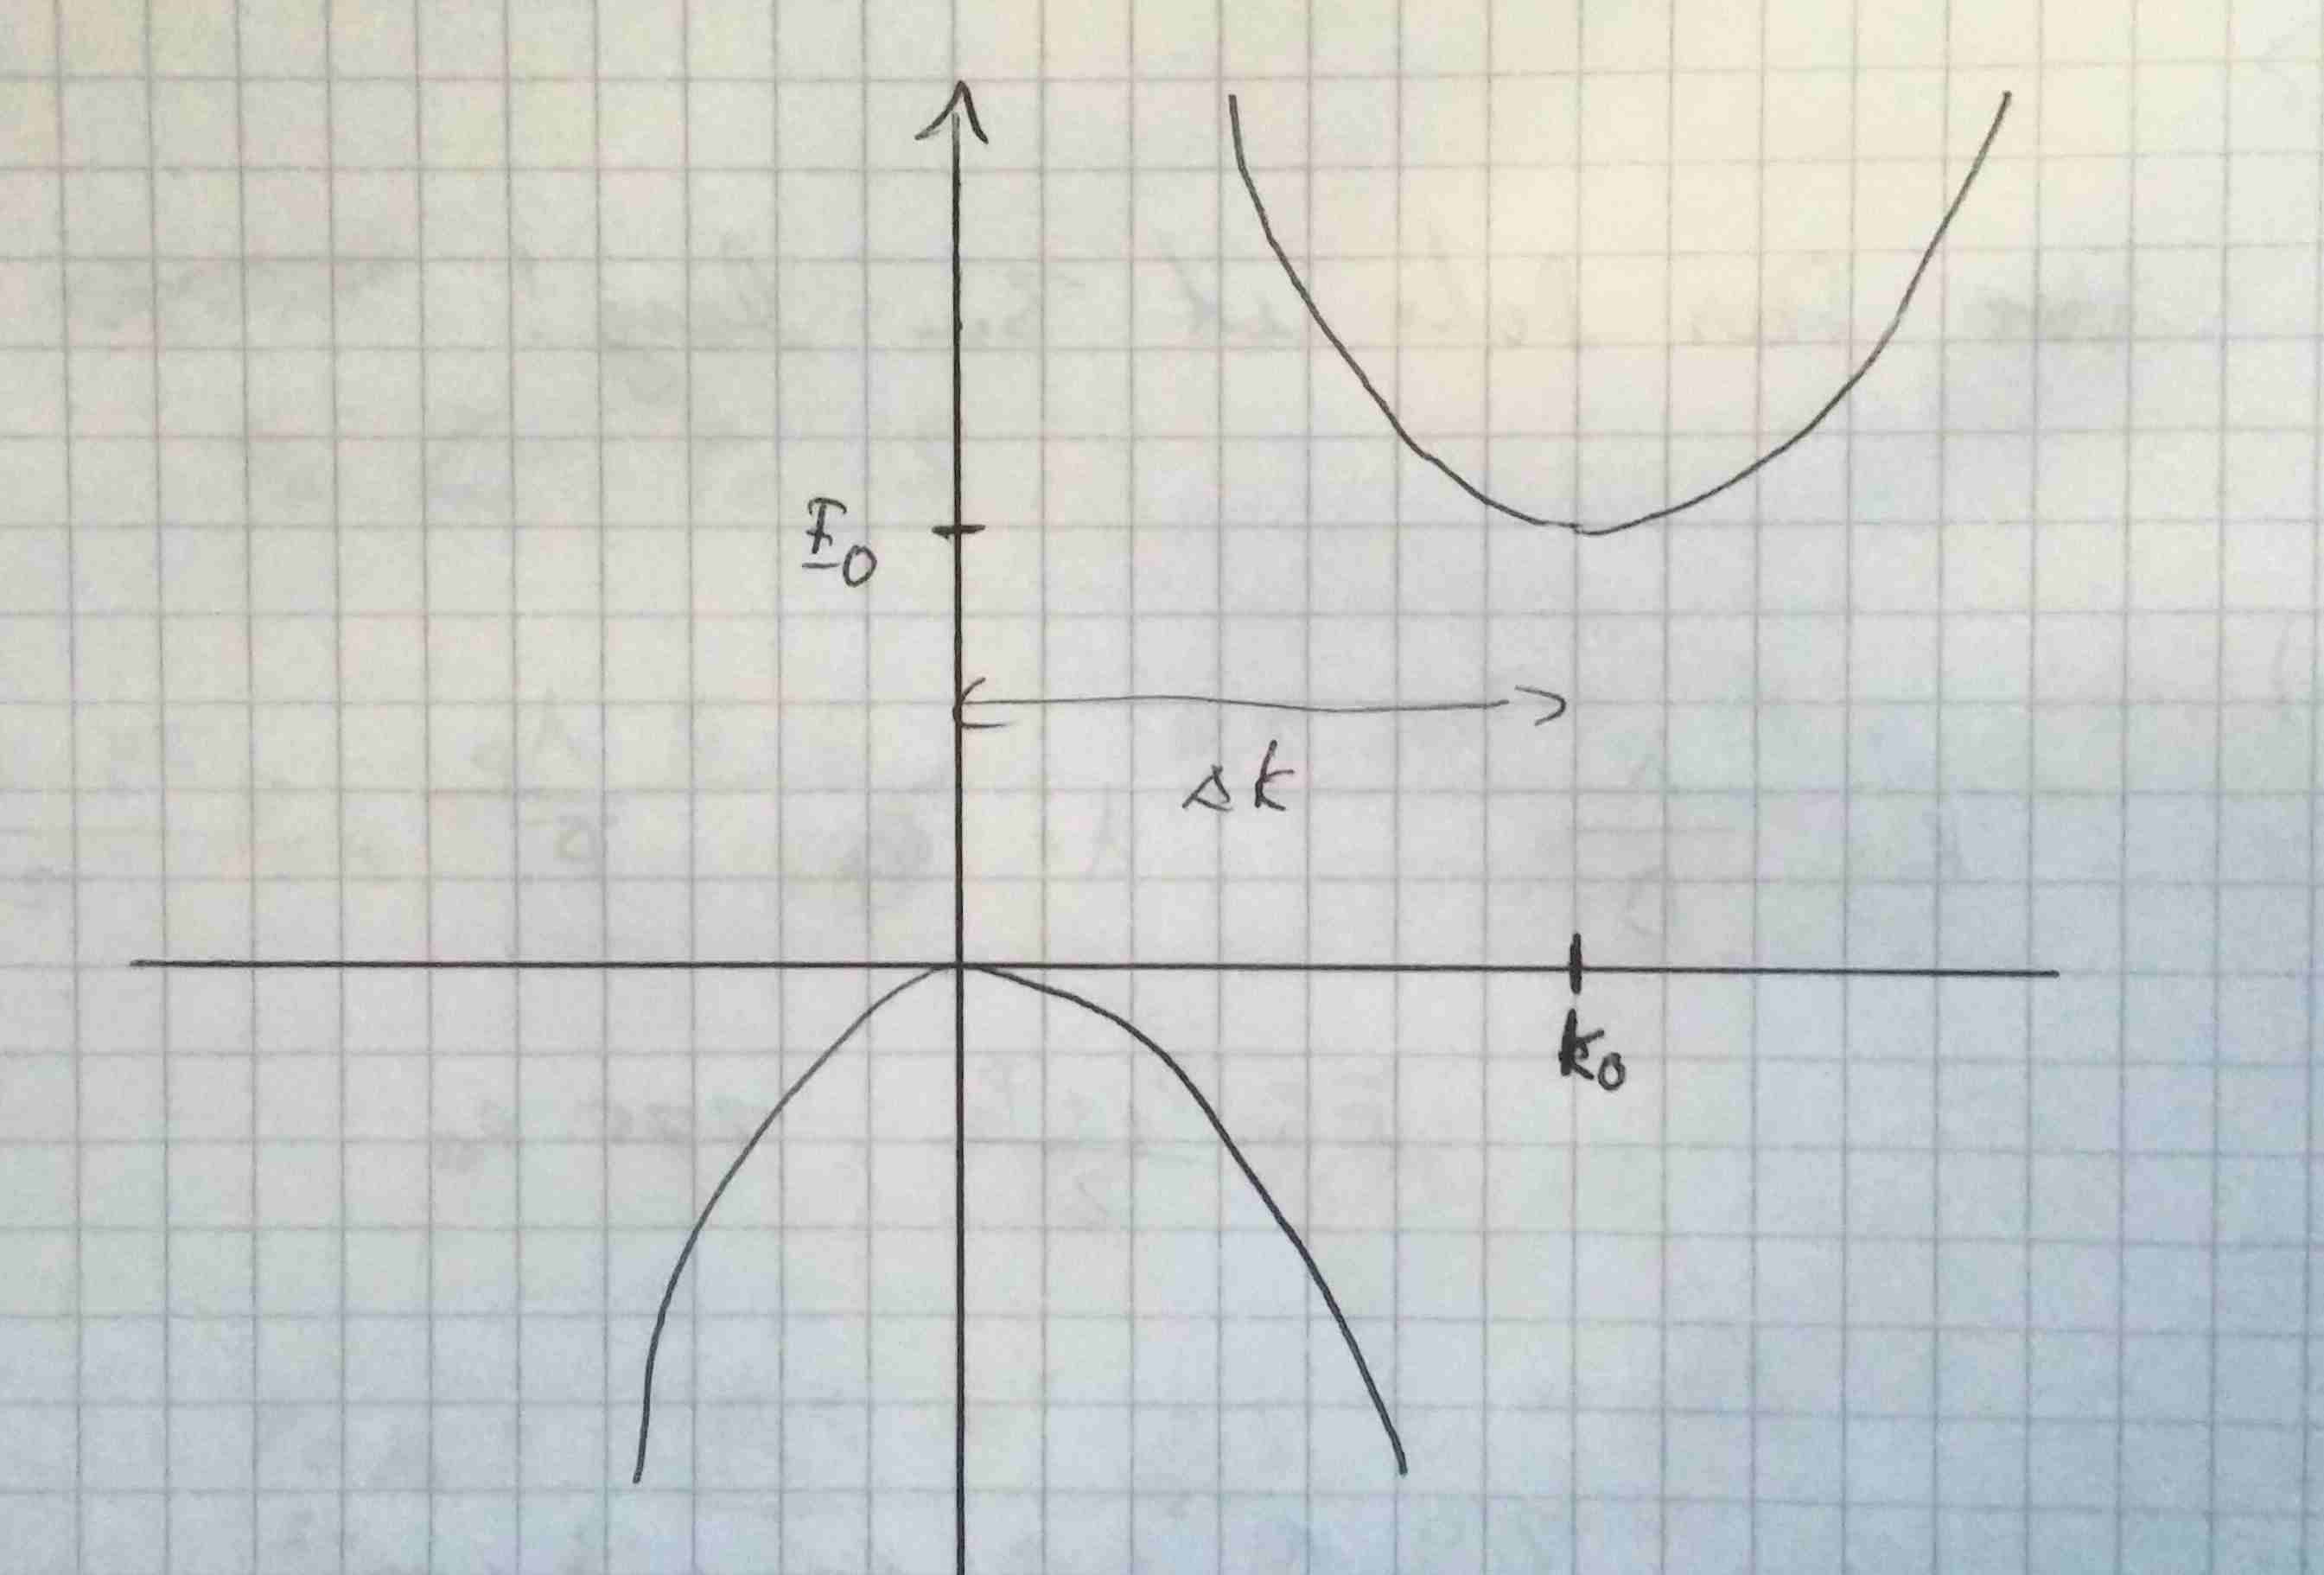
\includegraphics[scale=0.15]{A4_1.jpg}
\end{figure}

Wir müssen hier die Zustandsdichte über ein Intervall integrieren:

\begin{align*}
n &= \int_{0}^{1} D(E) \d E = \int_{0}^{1} \frac{4 \pi \cdot \left( 2m \right)^{3/2)} \cdot \sqrt{E}}{h^3} \\
&= \left. \frac{4 \pi \cdot \left( 2m \right)^{3/2}}{h^3} \frac{2}{3} \cdot E^{3/2}  \right|_0^1 \\
&= \frac{4\pi \left( 29,11 \cdot 10^{-31} \right)^{3/2}}{6,625 \cdot 10^{-34}} \cdot \frac{2}{3} \cdot \left( 1,6 \cdot 10^{-19} \right)^{3/2} = \unit[4,5 \cdot 10^{27}]{m^{-3}}
\end{align*}

Das sind dann Zustände pro Kubikmeter



\section{Aufgabe 5}

\subsection*{1D}

Wir definieren uns zunächst ein $\d z$:

\begin{align*}
\d z &= \frac{\text{Strecke}}{\text{Strecke für einen Zustand}} = \frac{\d k_x}{\frac{\pi}{a}} = \frac{a \d k_x}{\pi}
\intertext{Nun normieren wir $\d z$:}
\d z' &= \frac{\d z}{a} = \frac{\d k_x}{\pi}
\intertext{Nun bestimmen wir $k_x$:}
\d E &= \frac{\hbar^2 k_x}{m} \d k \\
\Leftrightarrow \d k &= \frac{m}{\hbar^2 k_x} \d E \\
\Leftrightarrow k_x &= \sqrt{\frac{2mE}{\hbar^2}}
\intertext{Nun können wir in die ursprüngliche Gleichung einsetzen:}
\d z' &= \frac{m \hbar }{\pi \hbar^2 \cdot \sqrt{2mE}} \d E = \frac{\sqrt{m}}{\pi \hbar \cdot \sqrt{2}} \cdot \frac{1}{\sqrt{E}} \d E
\end{align*}


\subsection*{2D}

Wir definieren uns wieder das $\d z$:

\begin{align*}
\d z &= \frac{\overbrace{2 \pi k \d k}^{\text{Fläche eines Kreisrings}}}{\left( \frac{\pi}{a} \right)} = \frac{2 \pi k a^2 \d k}{\pi^2}
\intertext{Wir normieren wieder:}
\d z' &= \frac{\d z}{a^2} = \frac{2 \pi k \d k}{\pi}
\intertext{Wir verwenden das $\d k$ aus dem vorigen Teil:}
&= \frac{2 \pi}{\pi^2} \cdot \sqrt{\frac{2mE}{\hbar^2}} \cdot \frac{m}{\hbar^2 \cdot k} \d E = \frac{2m}{\pi \hbar^2} \d E
\end{align*}

Wir sehen, das im zweidimensionalen Fall die Zustandsdichte konstant ist.


\section{Aufgabe 6}

\subsection*{a)}

Wir wissen das für die Energie der Elektonen $E = 3kT + E_F$ gilt. Wir können dies nun in die Zustandswahrscheinlichkeit einsetzen:

\begin{align*}
f_h(E) &= \frac{1}{1 + e^{\frac{E - E_F}{kT}}} = \frac{1}{1 + e^{\frac{3kT}{kT}}} = \frac{1}{1 + e^3} \\
&= 0,0474 = \unit[4,47]{\%}
\end{align*}

\subsection*{b)}

Hier sieht das ganze rech ähnlich aus:

\begin{align*}
f_h(E) = 1 - f(E) = \frac{1}{1 + e^{- \frac{E - E_F}{kT}}} = 0,0474 = \unit[4,74]{\%}
\end{align*}



schematisch sieht das ungefähr so aus:

\begin{figure}[h]
	\centering
	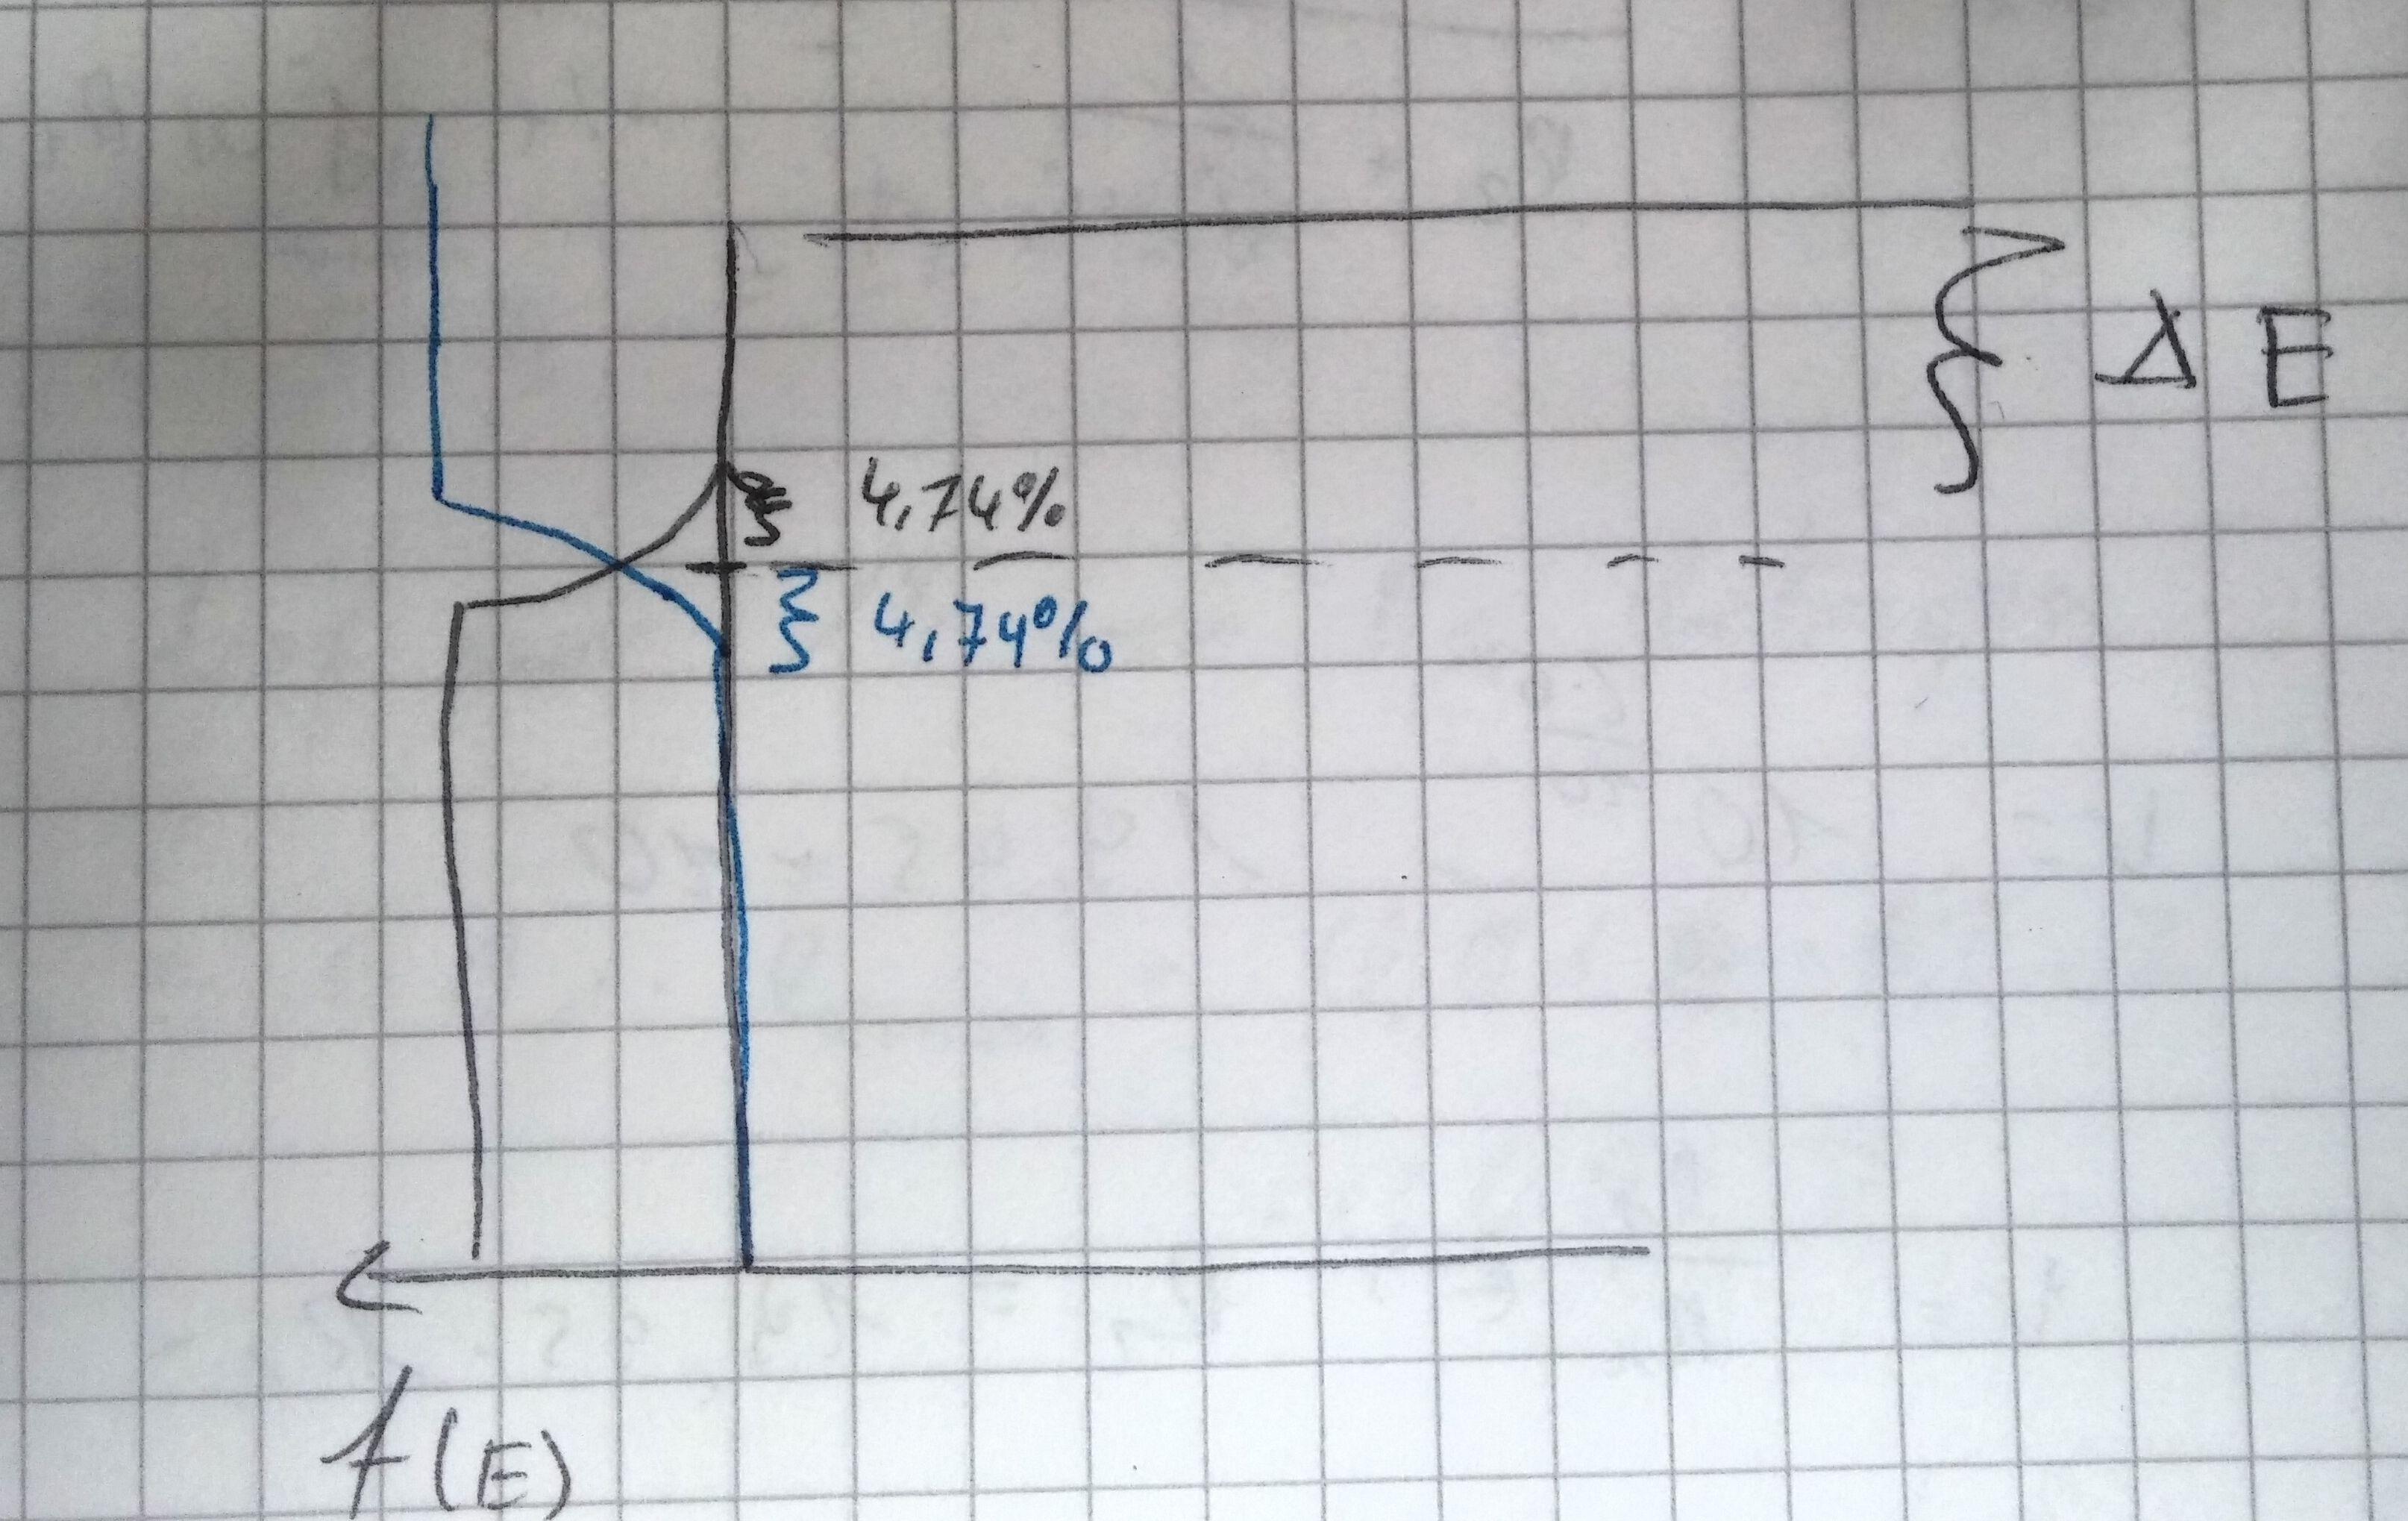
\includegraphics[scale=0.1]{A6_1.jpg}
\end{figure}


\section{Aufgabe 7}

Wir nehmen die Fermiverteilung von oben und setzen sie mit der Bolzmanverteilung gleich:

\begin{align*}
f(E) &= \frac{1}{1 + e^{\frac{E - E_F}{kT}}} = \frac{1}{1 + e^x} \qquad \text{mit} \qquad x = \frac{E - E_F}{kT} \\
\intertext{Wir setzen gleich:}
f_B(E) &= e^{- \frac{E - E_F}{kT}} = e^{-x} \\
\intertext{Dabei sollen nur $\unit[5]{\%}$ Fehler gemacht werden:}
\frac{5}{100} &= \frac{f_B(E) - f(E)}{f(E)} = \frac{e^{-x} + \frac{1}{1 + e^x}}{\frac{1}{1 + e^x}} = \frac{\frac{e^{-x} + e^0 - 1}{1 + e^x}}{\frac{1}{1 + e^x}} \\
\Leftrightarrow e^{-x} &= \frac{5}{100} \\
\Leftrightarrow x &= - \ln\left( \frac{5}{100} \right) \approx 3 \\
\Rightarrow \frac{E - E_F}{kT} &= 3 \qquad \rightarrow \qquad \Delta E = 3kT
\end{align*}


Verbildlicht sieht das ca so aus:

\begin{figure}[h]
	\centering
	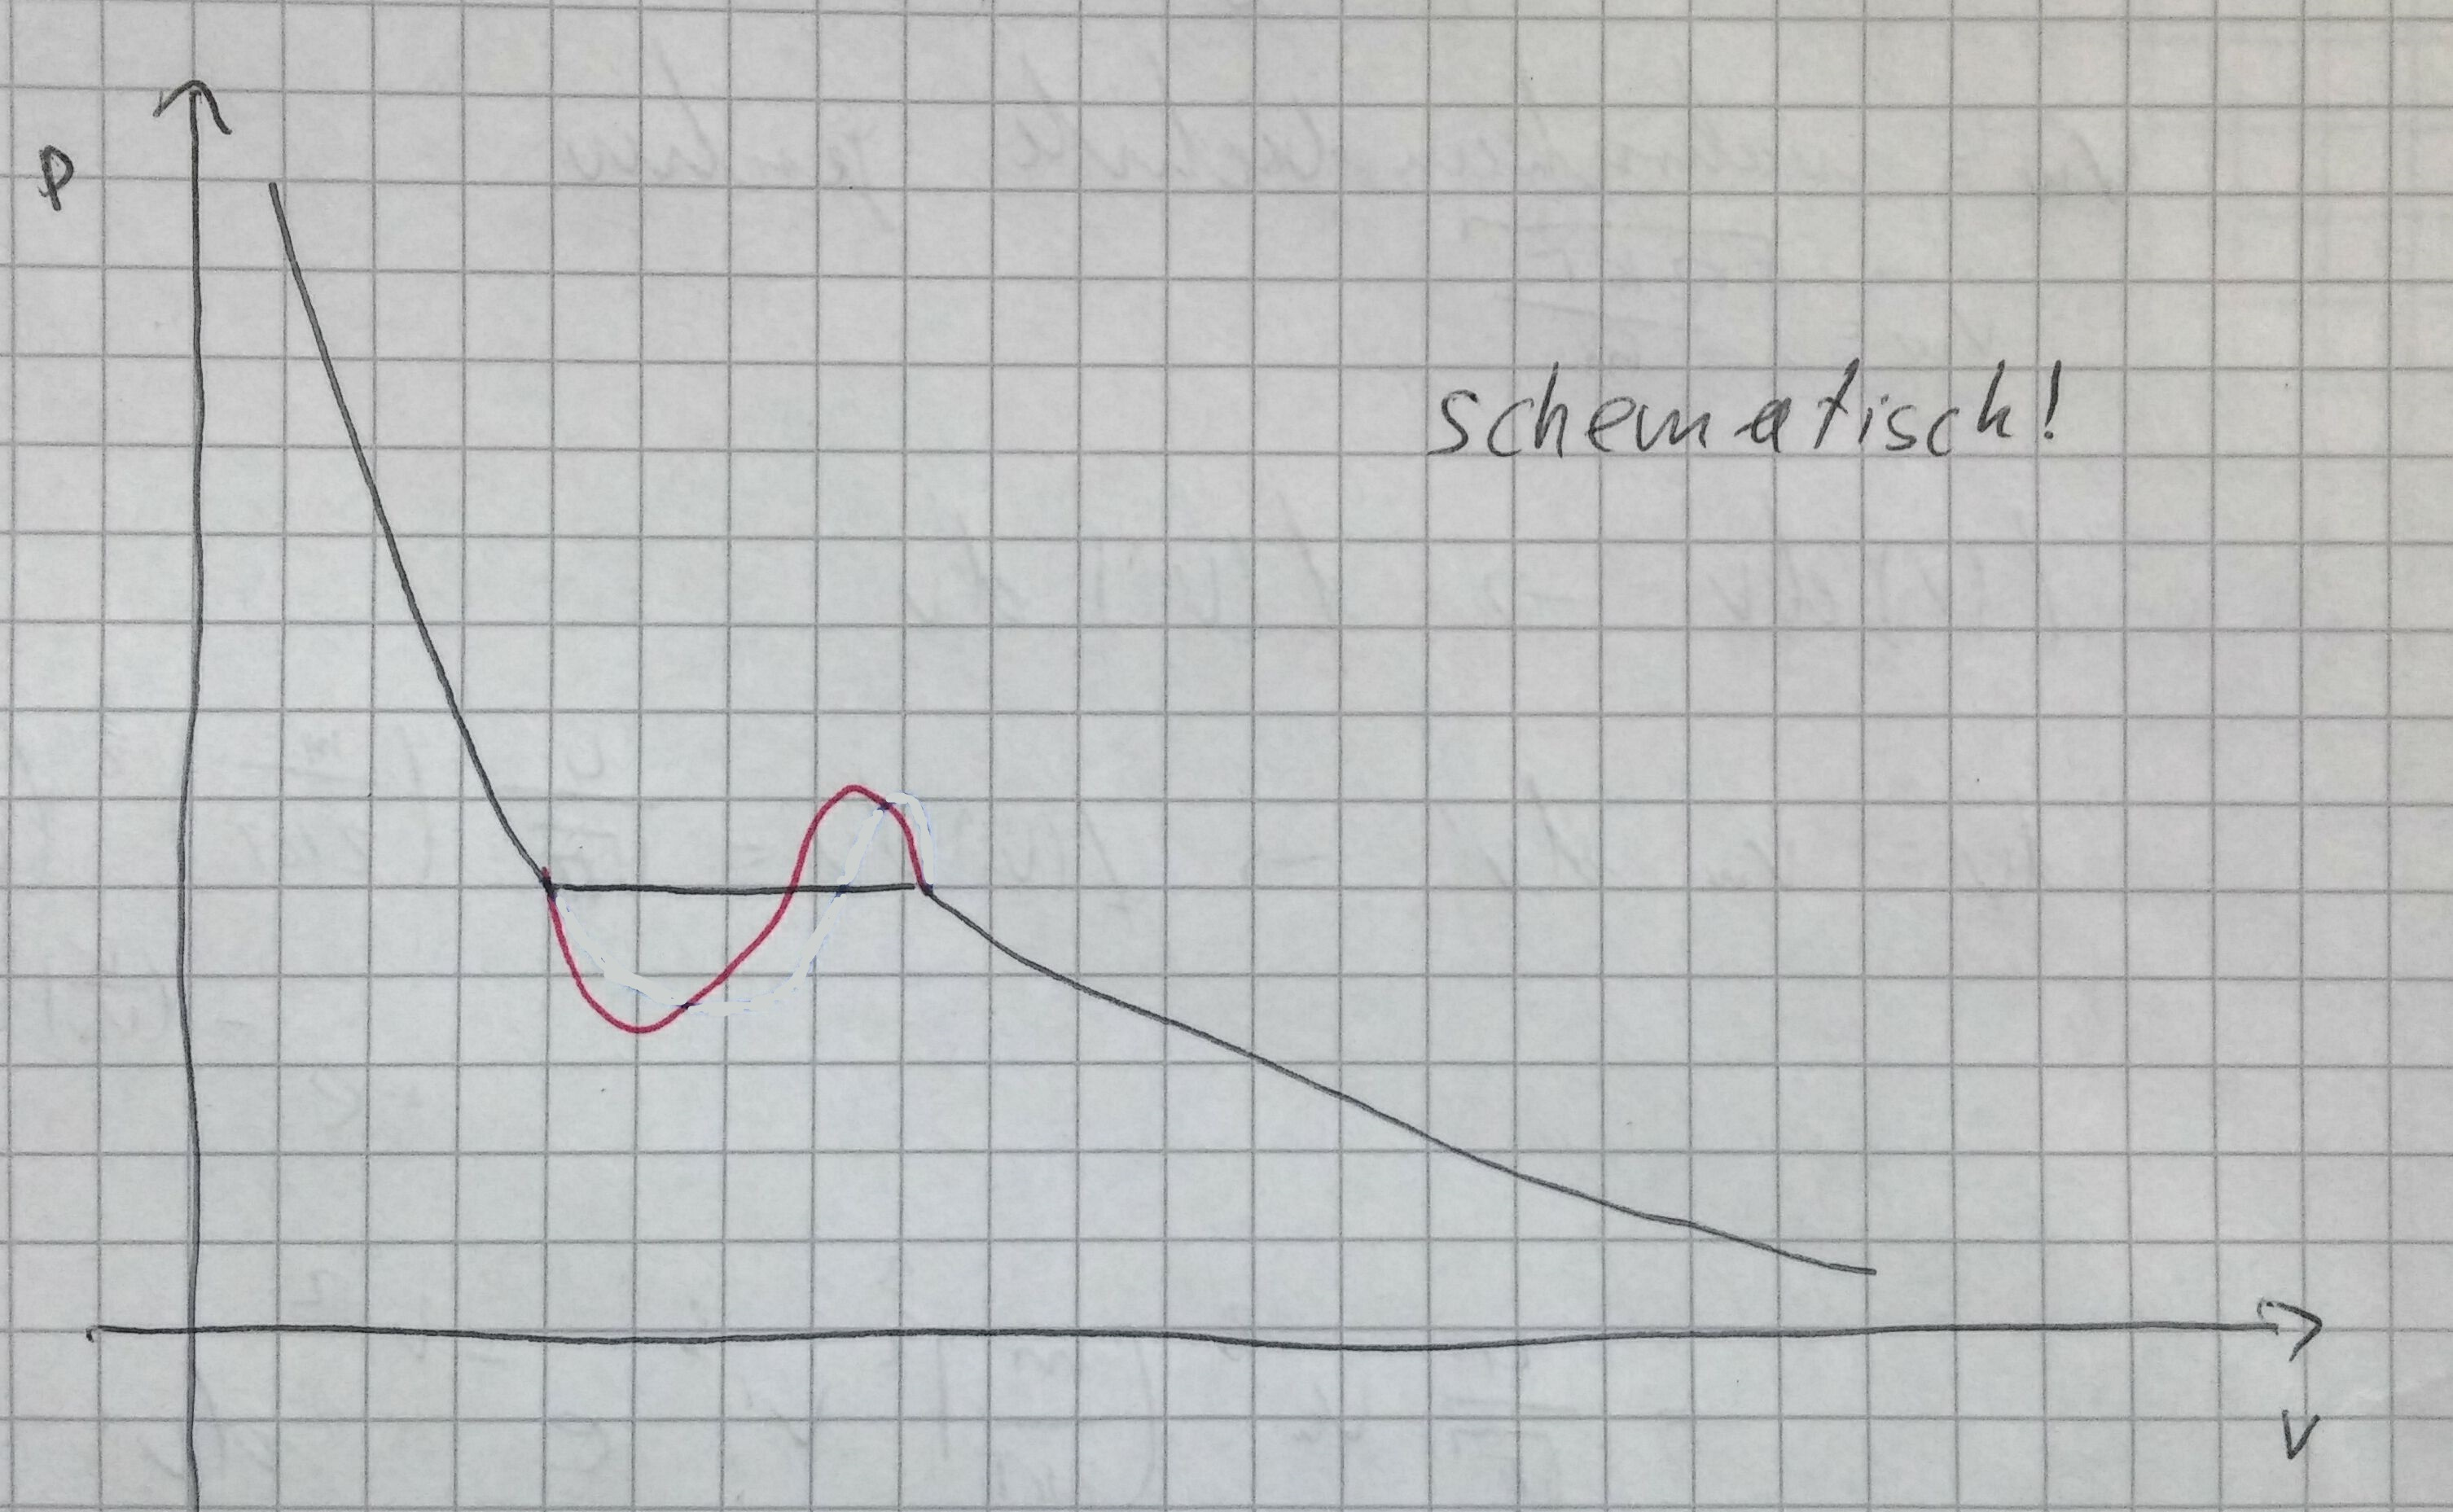
\includegraphics[scale=0.1]{A7_1.jpg}
\end{figure}


\newpage

\section{Aufgabe 8}

Alle Informationen sind in diesem Bild zusammengefasst:

\begin{figure}[h]
	\centering
	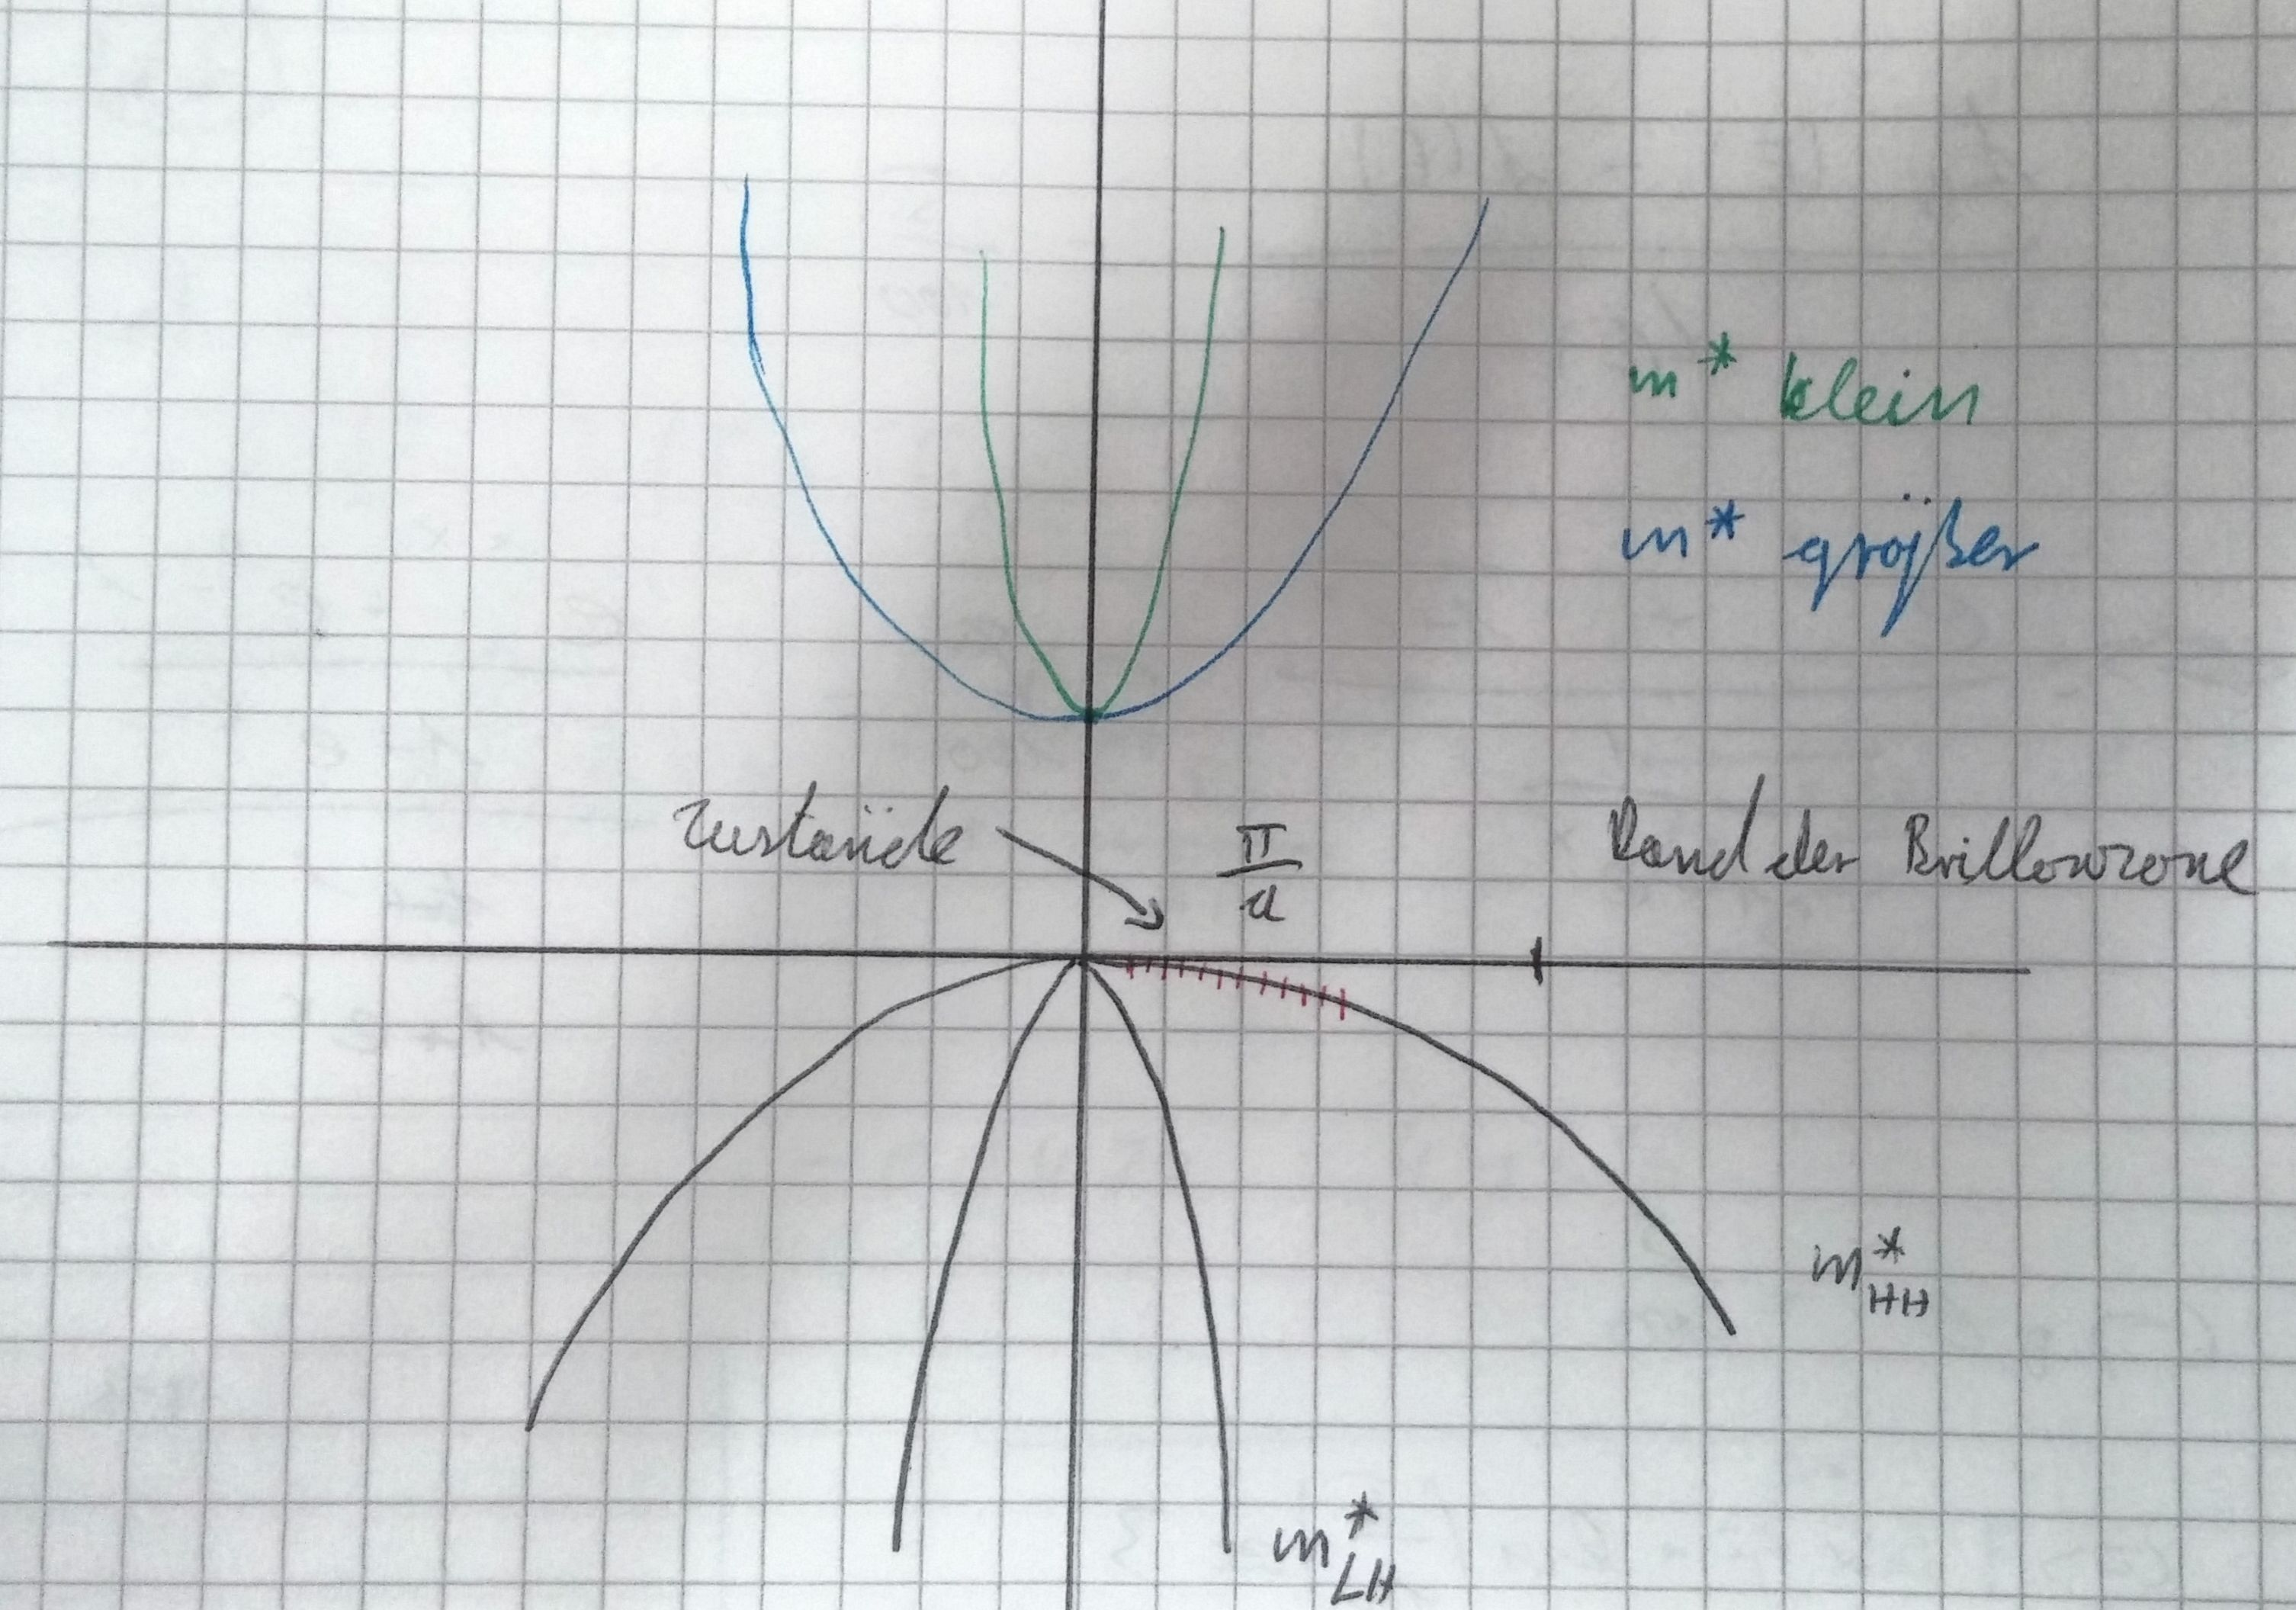
\includegraphics[scale=0.16]{A8_1.jpg}
\end{figure}











\end{document}